\documentclass[aspectratio=169,11pt]{ctexbeamer}

\usetheme{Madrid}
\usecolortheme{default}
\usefonttheme{professionalfonts}
\setbeamertemplate{navigation symbols}{}
\setbeamertemplate{caption}[numbered]
\setbeamertemplate{theorems}[numbered]

\usepackage{amsmath,amssymb,mathtools}
\usepackage{tikz}
\usetikzlibrary{arrows.meta,patterns,calc}
\usepackage{booktabs}
\usepackage{multicol}
\usepackage{graphicx}

% Unified Yingxing Beamer footer and visual style.
\newcommand{\huayinglogo}{assets/logo1.jpg}
\newcommand{\huayingslogan}{英行培优，成绩无忧；英行相伴，刮目相看}

\setbeamersize{text margin left=8mm,text margin right=8mm}
\setbeamerfont{frametitle}{size=\large}
\setbeamercolor{structure}{fg=blue!70!black}
\setbeamercolor{frametitle}{bg=blue!75!black,fg=white}
\setbeamercolor{block title}{bg=blue!10,fg=black}
\setbeamercolor{block body}{bg=blue!2,fg=black}
\setbeamercolor{author in head/foot}{bg=blue!8,fg=black}
\setbeamercolor{title in head/foot}{bg=blue!8,fg=black}

\setbeamertemplate{footline}{%
  \leavevmode%
  \hbox{%
    \begin{beamercolorbox}[wd=.12\paperwidth,ht=3.8ex,dp=1.2ex,center]{author in head/foot}%
      \includegraphics[height=2.9ex]{\huayinglogo}%
    \end{beamercolorbox}%
    \begin{beamercolorbox}[wd=.76\paperwidth,ht=3.8ex,dp=1.2ex,center]{title in head/foot}%
      \scriptsize \huayingslogan
    \end{beamercolorbox}%
    \begin{beamercolorbox}[wd=.12\paperwidth,ht=3.8ex,dp=1.2ex,right]{author in head/foot}%
      \scriptsize \insertframenumber/\inserttotalframenumber\hspace*{1em}
    \end{beamercolorbox}%
  }%
}

\title{连续函数的积分}
\subtitle{积分的定义、性质与典型例题}
\author{数学分析讲义}
\date{2026年4月18日}

\newtheorem{mydef}{定义}
\newtheorem{mythm}{定理}
\newtheorem{myprop}{性质}
\newtheorem{myex}{例}
\newtheorem{myrem}{注}

\newcommand{\dd}{\,\mathrm{d}}
\newcommand{\abs}[1]{\left|#1\right|}
\newcommand{\normp}{\lVert\pi\rVert}
\newcommand{\R}{\mathbb{R}}

\tikzset{
  axis/.style={-{Stealth[length=2mm]},thick},
  curve/.style={thick},
  shadearea/.style={fill=gray!35,draw=none},
  dashline/.style={dashed,thin}
}

\begin{document}

\begin{frame}
  \titlepage
\end{frame}

\begin{frame}{本讲目标}
  \begin{itemize}
    \item 从面积直观出发定义连续函数在闭区间上的积分；
    \item 用分段线性函数与黎曼和理解积分的极限过程；
    \item 掌握积分的线性、保序、可加性、估计与中值定理；
    \item 会用积分定义计算若干基本例子；
    \item 练习题与答案分开呈现，便于课堂讲解与课后核对。
  \end{itemize}
\end{frame}

\section{积分的定义}

\begin{frame}{面积直观}
  设 $f$ 为闭区间 $[a,b]$ 上的连续函数。若 $f(x)\ge 0$，则
  \[
    \int_a^b f(x)\dd x
  \]
  可以理解为曲线 $y=f(x)$、直线 $x=a,x=b$ 与 $x$ 轴围成的曲边梯形面积。

  \begin{center}
  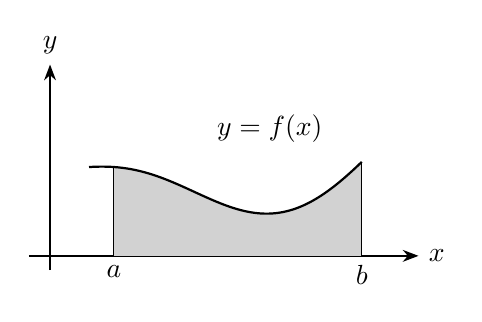
\begin{tikzpicture}[scale=0.9]
    \draw[axis] (-0.3,0) -- (5.2,0) node[right] {$x$};
    \draw[axis] (0,-0.2) -- (0,2.7) node[above] {$y$};
    \def\a{0.9}\def\b{4.4}
    \path[shadearea]
      (\a,0) -- plot[smooth,domain=\a:\b,samples=80]
      (\x,{0.8+0.2*(\x-2)^2/2+0.35*sin(80*\x)}) -- (\b,0) -- cycle;
    \draw[curve] plot[smooth,domain=0.55:4.4,samples=80]
      (\x,{0.8+0.2*(\x-2)^2/2+0.35*sin(80*\x)});
    \draw (\a,0) -- (\a,{0.8+0.2*(\a-2)^2/2+0.35*sin(80*\a)});
    \draw (\b,0) -- (\b,{0.8+0.2*(\b-2)^2/2+0.35*sin(80*\b)});
    \node[below] at (\a,0) {$a$};
    \node[below] at (\b,0) {$b$};
    \node at (3.1,1.8) {$y=f(x)$};
  \end{tikzpicture}
  \end{center}
\end{frame}

\begin{frame}{定义 1：常函数与线性函数的积分}
  \small
  \begin{mydef}[初等定义]
  先规定：
  \[
    \int_a^b c\dd x=c(b-a),
  \]
  若 $l(x)$ 是 $[a,b]$ 上的线性函数，则
  \[
    \int_a^b l(x)\dd x=\frac{l(a)+l(b)}2(b-a).
  \]
  \end{mydef}

  \begin{center}
  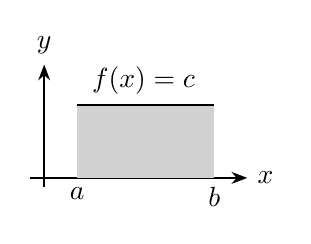
\begin{tikzpicture}[scale=0.6]
    \draw[axis] (-0.3,0)--(4.3,0) node[right]{$x$};
    \draw[axis] (0,-0.2)--(0,2.4) node[above]{$y$};
    \path[fill=gray!35] (0.7,0)--(0.7,1.55)--(3.6,1.55)--(3.6,0)--cycle;
    \draw[curve] (0.7,1.55)--(3.6,1.55);
    \node[above] at (2.1,1.55) {$f(x)=c$};
    \node[below] at (0.7,0) {$a$}; \node[below] at (3.6,0) {$b$};
  \end{tikzpicture}
  \hspace{1.1cm}
  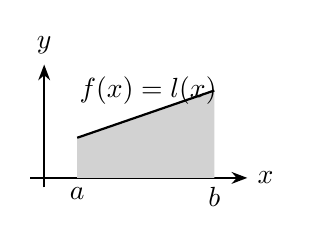
\begin{tikzpicture}[scale=0.6]
    \draw[axis] (-0.3,0)--(4.3,0) node[right]{$x$};
    \draw[axis] (0,-0.2)--(0,2.4) node[above]{$y$};
    \path[fill=gray!35] (0.7,0)--(0.7,0.85)--(3.6,1.85)--(3.6,0)--cycle;
    \draw[curve] (0.7,0.85)--(3.6,1.85);
    \node[above] at (2.2,1.35) {$f(x)=l(x)$};
    \node[below] at (0.7,0) {$a$}; \node[below] at (3.6,0) {$b$};
  \end{tikzpicture}
  \end{center}
\end{frame}

\begin{frame}{线性函数积分的三条基本性质}
  若 $f,g$ 都是 $[a,b]$ 上的线性函数，则
  \[
    \int_a^b\bigl(f(x)+g(x)\bigr)\dd x
    =\int_a^b f(x)\dd x+\int_a^b g(x)\dd x,
  \]
  \[
    \int_a^b\bigl(f(x)-g(x)\bigr)\dd x
    =\int_a^b f(x)\dd x-\int_a^b g(x)\dd x.
  \]
  若 $\abs{f(x)}\le M$，则
  \[
    \abs{\int_a^b f(x)\dd x}\le M(b-a).
  \]
  若 $c\in(a,b)$，则
  \[
    \int_a^b f(x)\dd x=\int_a^c f(x)\dd x+\int_c^b f(x)\dd x.
  \]
\end{frame}

\begin{frame}{定义 2：分段线性函数的积分}
  \footnotesize
  \begin{mydef}[分段线性积分]
  若存在分点
  \[
    a=x_0<x_1<\cdots<x_n=b,
  \]
  使得 $f$ 在每个 $[x_{i-1},x_i]$ 上都是线性函数，则定义
  \[
    \int_a^b f(x)\dd x
    =\sum_{i=1}^{n}\int_{x_{i-1}}^{x_i}f(x)\dd x.
  \]
  \end{mydef}
  分点的选取不影响积分值；线性、估计与区间可加性仍然成立。

  \begin{center}
  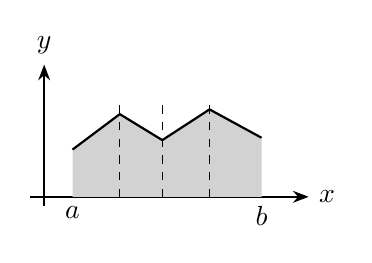
\begin{tikzpicture}[scale=0.6]
    \draw[axis] (-0.3,0)--(5.6,0) node[right]{$x$};
    \draw[axis] (0,-0.2)--(0,2.8) node[above]{$y$};
    \path[fill=gray!35] (0.6,0)--(0.6,1)--(1.6,1.75)--(2.5,1.2)--(3.5,1.85)--(4.6,1.25)--(4.6,0)--cycle;
    \draw[curve] (0.6,1)--(1.6,1.75)--(2.5,1.2)--(3.5,1.85)--(4.6,1.25);
    \foreach \x in {1.6,2.5,3.5} \draw[dashline] (\x,0)--(\x,2.05);
    \node[below] at (0.6,0){$a$}; \node[below] at (4.6,0){$b$};
  \end{tikzpicture}
  \end{center}
\end{frame}

\begin{frame}{用分段线性函数逼近连续函数}
  对 $[a,b]$ 作等分：
  \[
    x_i=a+\frac{i}{n}(b-a),\qquad i=0,1,\ldots,n.
  \]
  在每个 $[x_{i-1},x_i]$ 上，用连接
  \[
    (x_{i-1},f(x_{i-1})),\qquad (x_i,f(x_i))
  \]
  的线性函数 $l_i(x)$ 逼近 $f(x)$：
  \[
    l_i(x)=f(x_{i-1})+
    \frac{f(x_i)-f(x_{i-1})}{x_i-x_{i-1}}(x-x_{i-1}).
  \]
  定义分段线性函数 $f_n(x)=l_i(x)$，$x\in[x_{i-1},x_i]$。
\end{frame}

\begin{frame}{定理 1：分段线性逼近的一致收敛}
  \begin{mythm}[连续函数可由折线一致逼近]
  若 $f\in C[a,b]$，按上一页构造 $f_n$，则对任意 $\varepsilon>0$，存在 $N$，当 $n>N$ 时，
  \[
    \abs{f(x)-f_n(x)}<\varepsilon,\qquad x\in[a,b].
  \]
  \end{mythm}

  \begin{proof}
  由 $f$ 在闭区间上的一致连续性，取 $\delta>0$ 使
  $\abs{x'-x''}<\delta$ 时 $\abs{f(x')-f(x'')}<\varepsilon$。
  当 $(b-a)/n<\delta$，若 $x\in[x_{i-1},x_i]$，则
  \[
    \abs{f(x)-f_n(x)}
    \le \varepsilon\frac{x_i-x}{x_i-x_{i-1}}
       +\varepsilon\frac{x-x_{i-1}}{x_i-x_{i-1}}
    =\varepsilon.
  \]
  \end{proof}
\end{frame}

\begin{frame}{定义 3：连续函数的积分}
  \begin{mydef}[连续函数积分]
  对 $f\in C[a,b]$，令 $f_n$ 为上一节的分段线性逼近函数。定义
  \[
    \int_a^b f(x)\dd x
    =\lim_{n\to\infty}\int_a^b f_n(x)\dd x.
  \]
  \end{mydef}

  该定义与分段线性函数原有定义一致。由定理 1，
  \[
    \abs{\int_a^b f_m(x)\dd x-\int_a^b f_n(x)\dd x}
    \le 2\varepsilon(b-a),
  \]
  因而极限存在。
\end{frame}

\begin{frame}{等分黎曼和}
  根据分段线性逼近的定义，可得到
  \[
    \int_a^b f(x)\dd x
    =\lim_{n\to\infty}\sum_{i=1}^{n}
      \frac12\left[
      f\!\left(a+\frac{i-1}{n}(b-a)\right)
      +f\!\left(a+\frac{i}{n}(b-a)\right)\right]\frac{b-a}{n}.
  \]
  因端点项的影响在极限中消失，亦可写为
  \[
    \int_a^b f(x)\dd x
    =\lim_{n\to\infty}\frac{b-a}{n}
      \sum_{i=1}^{n}f\!\left(a+\frac{i}{n}(b-a)\right).
  \]

  \begin{myrem}
  这说明积分可看作“平均值 $\times$ 区间长度”。
  \end{myrem}
\end{frame}

\begin{frame}{任意取样点的黎曼和}
  由一致连续性，若
  \[
    \xi_i\in\left[a+\frac{i-1}{n}(b-a),\,a+\frac{i}{n}(b-a)\right],
  \]
  则仍有
  \[
    \int_a^b f(x)\dd x
    =\lim_{n\to\infty}\frac{b-a}{n}\sum_{i=1}^{n}f(\xi_i).
  \]
  更一般地，若
  \[
    \pi:\ a=x_0<x_1<\cdots<x_n=b,\qquad
    \normp=\max_i(x_i-x_{i-1}),
  \]
  则
  \[
    \int_a^b f(x)\dd x
    =\lim_{\normp\to0}\sum_{i=1}^{n}f(\xi_i)(x_i-x_{i-1}),
    \quad \xi_i\in[x_{i-1},x_i].
  \]
\end{frame}

\section{基本计算}

\begin{frame}{例 1：计算 $\int_a^b\cos x\dd x$}
  \begin{myex}
  由等分黎曼和，令 $h=(b-a)/n$。利用
  \[
    \sin\frac h2\cos(a+ih)
    =\frac12\left[
      \sin\!\left(a+\left(i+\frac12\right)h\right)
      -\sin\!\left(a+\left(i-\frac12\right)h\right)\right],
  \]
  有
  \[
  \begin{aligned}
    \int_a^b\cos x\dd x
    &=\lim_{n\to\infty}\frac{b-a}{n}\sum_{i=1}^{n}\cos(a+ih)\\
    &=\lim_{n\to\infty}
      \frac{b-a}{2n\sin\frac h2}
      \left[\sin\!\left(a+\left(n+\frac12\right)h\right)
      -\sin\!\left(a+\frac h2\right)\right]\\
    &=\sin b-\sin a.
  \end{aligned}
  \]
  \end{myex}
\end{frame}

\begin{frame}{例 2：计算 $\int_0^1 a^x\dd x$}
  \begin{myex}
  设 $a>0,\ a\ne1$。由等分黎曼和，
  \[
  \begin{aligned}
    \int_0^1 a^x\dd x
    &=\lim_{n\to\infty}\frac1n\sum_{i=1}^{n}a^{i/n}\\
    &=\lim_{n\to\infty}\frac1n\cdot
      a^{1/n}\frac{a-1}{a^{1/n}-1}.
  \end{aligned}
  \]
  令 $t=1/n$，则
  \[
    \int_0^1 a^x\dd x
    =\lim_{t\to0+}(a-1)\frac{t a^t}{a^t-1}
    =\frac{a-1}{\ln a}.
  \]
  \end{myex}
\end{frame}

\begin{frame}{例 3：计算 $\int_a^b\frac1{x^2}\dd x$}
  \begin{myex}
  设 $b>a>0$。在 $[x_{i-1},x_i]$ 上取
  \[
    \xi_i=\sqrt{x_{i-1}x_i}.
  \]
  则
  \[
  \begin{aligned}
    \int_a^b\frac1{x^2}\dd x
    &=\lim_{n\to\infty}\sum_{i=1}^{n}
      \frac1{\xi_i^2}(x_i-x_{i-1})\\
    &=\lim_{n\to\infty}\sum_{i=1}^{n}
      \frac{x_i-x_{i-1}}{x_{i-1}x_i}\\
    &=\lim_{n\to\infty}\sum_{i=1}^{n}
      \left(\frac1{x_{i-1}}-\frac1{x_i}\right)
      =\frac1a-\frac1b.
  \end{aligned}
  \]
  \end{myex}
\end{frame}

\section{积分的基本性质}

\begin{frame}{约定与性质 1：线性}
  约定：
  \[
    \int_a^a f(x)\dd x=0,\qquad
    \int_b^a f(x)\dd x=-\int_a^b f(x)\dd x.
  \]

  \begin{myprop}[线性]
  若 $f,g\in C[a,b]$，$\alpha,\beta\in\R$，则
  \[
    \int_a^b(\alpha f(x)+\beta g(x))\dd x
    =\alpha\int_a^b f(x)\dd x
    +\beta\int_a^b g(x)\dd x.
  \]
  \end{myprop}
\end{frame}

\begin{frame}[allowframebreaks]{性质 2：估计与保序}
  \small
  \begin{myprop}[绝对值估计]
  若 $\abs{f(x)}\le M$，$x\in[a,b]$，则
  \[
    \abs{\int_a^b f(x)\dd x}\le M(b-a).
  \]
  \end{myprop}

  \begin{myprop}[保序性]
  若 $f(x)\ge g(x)$，$x\in[a,b]$，则
  \[
    \int_a^b f(x)\dd x\ge\int_a^b g(x)\dd x.
  \]
  特别地，
  \[
    \abs{\int_a^b f(x)\dd x}\le\int_a^b\abs{f(x)}\dd x.
  \]
  \end{myprop}
\end{frame}

\begin{frame}{性质 3：区间可加性}
  \begin{myprop}[区间可加性]
  若 $f$ 连续，$a,b,c$ 属于定义域，则
  \[
    \int_a^c f(x)\dd x
    =\int_a^b f(x)\dd x+\int_b^c f(x)\dd x.
  \]
  \end{myprop}

  证明思路：先对 $a<b<c$ 取连续的分段线性函数 $\varphi,\psi$ 分别逼近
  $[a,b]$ 与 $[b,c]$ 上的 $f$，并令 $\varphi(b)=\psi(b)$。拼接成 $[a,c]$ 上的分段线性函数后，用估计
  \[
    \abs{\int_a^c f-\int_a^b f-\int_b^c f}
    \le 2\varepsilon(c-a)
  \]
  再令 $\varepsilon\to0$。
\end{frame}

\begin{frame}{性质 4：非负函数的积分}
  \begin{myprop}[非负性]
  若 $f\in C[a,b]$ 且 $f(x)\ge0$，则
  \[
    \int_a^b f(x)\dd x\ge0.
  \]
  且等号成立当且仅当 $f\equiv0$。
  \end{myprop}

  若存在 $x_0\in[a,b]$ 使 $f(x_0)>0$，由连续性，存在 $[c,d]\subset[a,b]$，
  \[
    f(x)>\frac12 f(x_0),\qquad x\in[c,d].
  \]
  于是
  \[
    \int_a^b f(x)\dd x
    \ge\int_c^d f(x)\dd x
    \ge \frac{f(x_0)}2(d-c)>0.
  \]
\end{frame}

\begin{frame}{例 4：积分函数是 Lipschitz 函数}
  \footnotesize
  \begin{myex}
  设 $f\in C[a,b]$，$c\in[a,b]$，定义
  \[
    F(x)=\int_c^x f(t)\dd t,\qquad x\in[a,b].
  \]
  则 $F$ 为 Lipschitz 函数。
  \end{myex}

  \begin{proof}
  因 $f$ 连续，存在 $M>0$ 使 $\abs{f(x)}\le M$。若 $x_1\le x_2$，则
  \[
  \begin{aligned}
    \abs{F(x_2)-F(x_1)}
    &=\abs{\int_{x_1}^{x_2}f(x)\dd x}\\
    &\le\int_{x_1}^{x_2}\abs{f(x)}\dd x
    \le M\abs{x_2-x_1}.
  \end{aligned}
  \]
  \end{proof}
\end{frame}

\begin{frame}{例 5：与任意连续函数正交则恒为零}
  \begin{myex}
  若 $f\in C[a,b]$，并且对任意 $g\in C[a,b]$ 都有
  \[
    \int_a^b f(x)g(x)\dd x=0,
  \]
  则 $f\equiv0$。
  \end{myex}

  \begin{proof}
  取 $g=f$，得
  \[
    \int_a^b f^2(x)\dd x=0.
  \]
  因 $f^2\ge0$ 且连续，由非负性中的等号条件知 $f^2\equiv0$，故 $f\equiv0$。
  \end{proof}
\end{frame}

\section{变量代换与中值定理}

\begin{frame}{积分中的简单变量代换}
  由黎曼和表达式可直接得到：
  \[
    \int_a^b f(x)\dd x=\int_{a-c}^{b-c}f(t+c)\dd t,
  \]
  以及当 $\alpha\ne0$ 时，
  \[
    \int_a^b f(x)\dd x
    =\alpha\int_{a/\alpha}^{b/\alpha}f(\alpha t)\dd t.
  \]

  \begin{myex}
  若 $x>0$，$a>0$ 且 $a\ne1$，则
  \[
    \int_0^x a^t\dd t
    =x\int_0^1 (a^x)^s\dd s
    =x\frac{a^x-1}{\ln a^x}
    =\frac{a^x-1}{\ln a}.
  \]
  \end{myex}
\end{frame}

\begin{frame}{定理 2：积分中值定理}
  \footnotesize
  \begin{mythm}[积分中值定理]
  设 $f,g\in C[a,b]$，且 $g$ 不变号，则存在 $\xi\in[a,b]$，使
  \[
    \int_a^b f(x)g(x)\dd x
    =f(\xi)\int_a^b g(x)\dd x.
  \]
  \end{mythm}

  \begin{proof}
  不妨设 $g\ge0$。令 $m,M$ 为 $f$ 在 $[a,b]$ 上的最小值和最大值，则
  \[
    m g(x)\le f(x)g(x)\le M g(x).
  \]
  积分得
  \[
    m\le
    \frac{\int_a^b f(x)g(x)\dd x}{\int_a^b g(x)\dd x}
    \le M
  \]
  （若 $\int g=0$，结论显然）。由介值定理即得。
  \end{proof}
\end{frame}

\begin{frame}{推论：平均值形式}
  取 $g\equiv1$，存在 $\xi\in[a,b]$ 使
  \[
    f(\xi)=\frac1{b-a}\int_a^b f(x)\dd x,
  \]
  或
  \[
    \int_a^b f(x)\dd x=f(\xi)(b-a).
  \]
  因此 $f(\xi)$ 是 $f$ 在 $[a,b]$ 上的平均值。
\end{frame}

\section{进一步例子}

\begin{frame}{例 6：一个和式极限}
  \begin{myex}
  求
  \[
    \lim_{n\to\infty}\left(\frac1{n+1}+\frac1{n+2}+\cdots+\frac1{2n}\right).
  \]
  \end{myex}

  \[
  \begin{aligned}
    \frac1{n+1}+\cdots+\frac1{2n}
    &=\frac1n\left(\frac1{1+\frac1n}+\cdots+\frac1{1+\frac nn}\right)\\
    &\longrightarrow\int_0^1\frac1{1+x}\dd x
    =\int_1^2\frac1t\dd t=\ln2.
  \end{aligned}
  \]
\end{frame}

\begin{frame}{例 7：至少两个零点}
  \small
  \begin{myex}
  设 $f\in C[a,b]$，且
  \[
    \int_a^b f(x)\dd x=\int_a^b x f(x)\dd x=0.
  \]
  则 $f$ 在 $(a,b)$ 内至少有两个零点。
  \end{myex}

  若 $f$ 在 $(a,b)$ 内没有零点，则 $f$ 恒正或恒负，导致 $\int_a^b f\ne0$，矛盾。
  若只有一个内部零点 $x_0$，则 $(x-x_0)f(x)$ 在 $(a,b)$ 上同号，且不恒为零，所以
  \[
    \int_a^b (x-x_0)f(x)\dd x>0\quad\text{或}<0.
  \]
  但
  \[
    \int_a^b (x-x_0)f(x)\dd x
    =\int_a^b x f(x)\dd x-x_0\int_a^b f(x)\dd x=0,
  \]
  矛盾。
\end{frame}

\begin{frame}{定理 3：Young 不等式}
  \begin{mythm}[Young 不等式的积分形式]
  设 $f$ 是 $[0,+\infty)$ 上的严格递增连续函数，$f(0)=0$，$f^{-1}$ 为反函数。则 $a,b>0$ 时
  \[
    ab\le\int_0^a f(x)\dd x+\int_0^b f^{-1}(y)\dd y.
  \]
  等号成立当且仅当 $b=f(a)$。
  \end{mythm}

  \begin{center}
  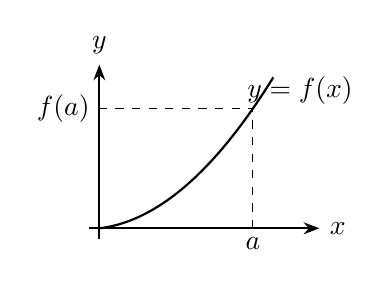
\begin{tikzpicture}[scale=0.65]
    \draw[axis] (-0.2,0)--(4.3,0) node[right]{$x$};
    \draw[axis] (0,-0.2)--(0,3.2) node[above]{$y$};
    \draw[curve] plot[smooth,domain=0:3.4,samples=80] (\x,{0.22*\x*\x+0.12*\x});
    \draw[dashline] (3,0)--(3,2.34)--(0,2.34);
    \node[right] at (2.7,2.7){$y=f(x)$};
    \node[below] at (3,0){$a$}; \node[left] at (0,2.34){$f(a)$};
  \end{tikzpicture}
  \hspace{0.8cm}
  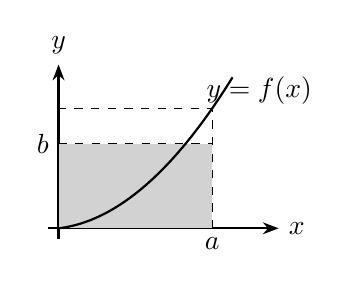
\begin{tikzpicture}[scale=0.65]
    \draw[axis] (-0.2,0)--(4.3,0) node[right]{$x$};
    \draw[axis] (0,-0.2)--(0,3.2) node[above]{$y$};
    \path[fill=gray!35] (0,0)--(3,0)--(3,1.65)--(0,1.65)--cycle;
    \draw[curve] plot[smooth,domain=0:3.4,samples=80] (\x,{0.22*\x*\x+0.12*\x});
    \draw[dashline] (3,0)--(3,2.34)--(0,2.34);
    \draw[dashline] (0,1.65)--(3,1.65);
    \node[right] at (2.7,2.7){$y=f(x)$};
    \node[below] at (3,0){$a$}; \node[left] at (0,1.65){$b$};
  \end{tikzpicture}
  \end{center}
\end{frame}

\begin{frame}{Young 不等式的常用推论}
  取
  \[
    f(x)=x^{p-1}\quad(p>1),
  \]
  则
  \[
    f^{-1}(y)=y^{q-1},\qquad \frac1p+\frac1q=1.
  \]
  Young 不等式给出
  \[
    ab\le\frac{a^p}{p}+\frac{b^q}{q},\qquad a,b\ge0.
  \]
  当 $p=q=2$ 时，就是
  \[
    ab\le\frac{a^2+b^2}{2}.
  \]
\end{frame}

\begin{frame}{定理 4：Hölder 不等式}
  \begin{mythm}[Hölder 不等式]
  若 $f,g\in C[a,b]$，$p>1$，$\frac1p+\frac1q=1$，则
  \[
    \int_a^b\abs{f(x)g(x)}\dd x
    \le
    \left(\int_a^b\abs{f(x)}^p\dd x\right)^{1/p}
    \left(\int_a^b\abs{g(x)}^q\dd x\right)^{1/q}.
  \]
  \end{mythm}
  等号成立当且仅当存在常数 $c$，使
  \[
    \abs{f(x)}^p=c\abs{g(x)}^q.
  \]
  证明可将 Young 不等式应用于归一化后的
  $\abs{f(x)}$ 与 $\abs{g(x)}$，再在 $[a,b]$ 上积分。
\end{frame}

\begin{frame}{例 8：周期振荡函数的积分}
  \small
  \begin{myex}
  设 $f\in C[a,b]$，$g$ 是周期为 $T$ 的连续周期函数，则
  \[
    \lim_{n\to\infty}\int_a^b f(x)g(nx)\dd x
    =\frac1T\int_a^b f(x)\dd x\int_0^T g(x)\dd x.
  \]
  \end{myex}
  证明中可先将 $g$ 减去其周期平均值，化为
  $\int_0^T g(x)\dd x=0$ 的情形，再利用 $f$ 的一致连续性与
  \[
    \abs{\int_0^c g(nx)\dd x}\le \frac{T}{n}\max\abs{g}
  \]
  控制每个小区间上的振荡贡献。

  \begin{center}
  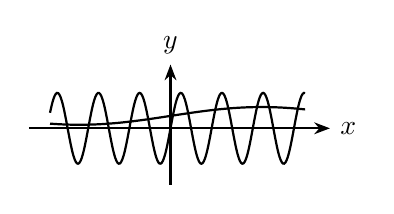
\begin{tikzpicture}[scale=0.45]
    \draw[axis] (-4,0)--(4.5,0) node[right]{$x$};
    \draw[axis] (0,-1.6)--(0,1.8) node[above]{$y$};
    \draw[curve] plot[smooth,domain=-3.4:3.8,samples=220] (\x,{sin(310*\x)});
    \draw[curve] plot[smooth,domain=-3.4:3.8,samples=80] (\x,{0.35+0.25*sin(35*\x)});
  \end{tikzpicture}
  \end{center}
\end{frame}

\section{习题}

\begin{frame}{习题 1--4}
  \begin{enumerate}
    \item 若 $f$ 本身是分段线性的连续函数，证明等分区间分段线性逼近所得积分极限与分段线性积分一致。
    \item 按定义计算 $\displaystyle\int_a^b\sin x\dd x$。
    \item 设 $b>a>0,\ \alpha\ne-1$，按定义求 $\displaystyle\int_a^b x^\alpha\dd x$。
    \item 设
    \[
      f(x)=\int_1^x\frac{\dd t}{t},\qquad x>0.
    \]
    不借助对数函数，证明 $f(xy)=f(x)+f(y)$。
  \end{enumerate}
\end{frame}

\begin{frame}{答案 1}
  将分段线性函数的原分点与等分分点合并，得到更细的分割。由分段线性积分的分点无关性，任意细化不改变积分值。

  等分折线逼近 $f_n$ 在每个足够小的区间上与 $f$ 的误差趋于 $0$。于是
  \[
    \abs{\int_a^b f_n-\int_a^b f}
    \le (b-a)\max_{[a,b]}\abs{f_n-f}\to0.
  \]
  因此按等分逼近定义得到的积分极限，等于原来的分段线性积分。
\end{frame}

\begin{frame}{答案 2}
  令 $h=(b-a)/n$。由等分黎曼和，
  \[
    \int_a^b\sin x\dd x
    =\lim_{n\to\infty}h\sum_{i=1}^{n}\sin(a+ih).
  \]
  利用
  \[
    2\sin\frac h2\sin(a+ih)
    =\cos\!\left(a+\left(i-\frac12\right)h\right)
     -\cos\!\left(a+\left(i+\frac12\right)h\right),
  \]
  得
  \[
    \int_a^b\sin x\dd x
    =-\cos b+\cos a.
  \]
\end{frame}

\begin{frame}{答案 3}
  取几何分割
  \[
    a,\ aq,\ aq^2,\ldots,aq^n=b,\qquad q=\left(\frac ba\right)^{1/n}.
  \]
  在区间 $[aq^{i-1},aq^i]$ 中取 $\xi_i$ 使
  \[
    \xi_i^\alpha=\frac{(aq^i)^{\alpha+1}-(aq^{i-1})^{\alpha+1}}
    {(\alpha+1)(aq^i-aq^{i-1})}.
  \]
  则黎曼和望远镜相消，得到
  \[
    \int_a^b x^\alpha\dd x
    =\frac{b^{\alpha+1}-a^{\alpha+1}}{\alpha+1}.
  \]
\end{frame}

\begin{frame}{答案 4}
  对 $x,y>0$，
  \[
    f(xy)=\int_1^{xy}\frac{\dd t}{t}
    =\int_1^x\frac{\dd t}{t}+\int_x^{xy}\frac{\dd t}{t}.
  \]
  第二项作变量代换 $t=xs$：
  \[
    \int_x^{xy}\frac{\dd t}{t}
    =\int_1^y\frac{x\dd s}{xs}
    =\int_1^y\frac{\dd s}{s}=f(y).
  \]
  故 $f(xy)=f(x)+f(y)$。
\end{frame}

\begin{frame}{习题 5--8}
  \begin{enumerate}
    \setcounter{enumi}{4}
    \item 若 $g$ 为连续周期函数，周期为 $T$，证明当 $b-a=T$ 时
    \[
      \int_a^b g(x)\dd x=\int_0^T g(x)\dd x.
    \]
    \item 证明 $F(x)=\displaystyle\int_0^x\frac{\dd t}{1+t^2}$ 关于 $x>0$ 有界。
    \item 说明积分中值定理中的点 $\xi$ 可取在开区间 $(a,b)$ 中。
    \item 若 $f\in C[a,b]$，且对任意满足 $g(a)=g(b)=0$ 的连续函数 $g$ 都有
    \[
      \int_a^b f(x)g(x)\dd x=0,
    \]
    证明 $f=0$。
  \end{enumerate}
\end{frame}

\begin{frame}{答案 5}
  由周期性 $g(x+T)=g(x)$，作代换 $x=t+a$：
  \[
    \int_a^{a+T}g(x)\dd x=\int_0^T g(t+a)\dd t.
  \]
  对任意 $c$，函数 $G(c)=\int_c^{c+T}g(x)\dd x$ 满足
  \[
    G(c+h)-G(c)=\int_{c+T}^{c+T+h}g-\int_c^{c+h}g=0
  \]
  在极限意义下恒为零，故 $G$ 为常数。取 $c=0$ 即得结论。
\end{frame}

\begin{frame}{答案 6}
  对 $x>0$，
  \[
    0\le F(x)=\int_0^x\frac{\dd t}{1+t^2}.
  \]
  当 $0<x\le1$ 时，$F(x)\le x\le1$。当 $x>1$ 时，
  \[
    F(x)=\int_0^1\frac{\dd t}{1+t^2}
      +\int_1^x\frac{\dd t}{1+t^2}
    \le 1+\int_1^x\frac{\dd t}{t^2}
    \le 2.
  \]
  因此 $F(x)$ 在 $(0,+\infty)$ 上有界。
\end{frame}

\begin{frame}{答案 7}
  若 $f$ 在 $[a,b]$ 上非常值，则中值定理中的数
  \[
    A=\frac{\int_a^b f(x)g(x)\dd x}{\int_a^b g(x)\dd x}
  \]
  位于 $f$ 的最小值与最大值之间。连续函数在端点之外也会取到所有严格介于最小值和最大值之间的值，所以可取 $\xi\in(a,b)$。

  若 $f$ 为常值，则任取 $\xi\in(a,b)$ 均可。
\end{frame}

\begin{frame}{答案 8}
  已知测试函数只要求端点为零。取
  \[
    g(x)=(x-a)(b-x)f(x),
  \]
  则 $g\in C[a,b]$ 且 $g(a)=g(b)=0$。于是
  \[
    0=\int_a^b f(x)g(x)\dd x
    =\int_a^b (x-a)(b-x)f^2(x)\dd x.
  \]
  被积函数非负且连续，在 $(a,b)$ 内权重 $(x-a)(b-x)>0$。故 $f(x)=0$，$x\in(a,b)$。由连续性，端点也为零。
\end{frame}

\begin{frame}{习题 9--10}
  \begin{enumerate}
    \setcounter{enumi}{8}
    \item 若对任意满足 $\int_a^b g(x)\dd x=0$ 的连续函数 $g$，都有
    \[
      \int_a^b f(x)g(x)\dd x=0,
    \]
    证明 $f$ 为常数。
    \item 设 $f\in C[a,b]$，且
    \[
      \int_a^b f=\int_a^b xf=\int_a^b x^2f=0,
    \]
    证明 $f$ 在 $(a,b)$ 内至少有三个零点。
  \end{enumerate}
\end{frame}

\begin{frame}{习题 11--12}
  \begin{enumerate}
    \setcounter{enumi}{10}
    \item 若 $f$ 在 $[a,b]$ 上单调递增，证明
    \[
      (a+b)\int_a^b f(x)\dd x\le2\int_a^b x f(x)\dd x.
    \]
    \item 设 $f\in C[a,b]$，证明
    \[
      \lim_{n\to\infty}\left[\int_a^b\abs{f(x)}^n\dd x\right]^{1/n}
      =\max_{x\in[a,b]}\abs{f(x)}.
    \]
  \end{enumerate}
\end{frame}

\begin{frame}{答案 9}
  设
  \[
    C=\frac1{b-a}\int_a^b f(x)\dd x.
  \]
  取 $g=f-C$，则
  \[
    \int_a^b g(x)\dd x=0.
  \]
  由条件，
  \[
    0=\int_a^b f(x)(f(x)-C)\dd x
    =\int_a^b (f(x)-C)^2\dd x
      +C\int_a^b(f(x)-C)\dd x.
  \]
  第二项为零，所以 $\int_a^b(f-C)^2=0$，故 $f\equiv C$。
\end{frame}

\begin{frame}{答案 10}
  反设 $f$ 在 $(a,b)$ 内至多有两个零点。可取二次多项式
  \[
    p(x)=(x-\alpha)(x-\beta)
  \]
  使 $p(x)f(x)$ 在 $(a,b)$ 内不变号且不恒为零（若零点少于两个，可令其中某些根放在区间外或重复）。

  因 $p(x)=x^2-(\alpha+\beta)x+\alpha\beta$，由三个积分条件得
  \[
    \int_a^b p(x)f(x)\dd x=0.
  \]
  但 $p f$ 连续不变号且不恒为零，其积分不能为零，矛盾。
  因此 $f$ 至少有三个内部零点。
\end{frame}

\begin{frame}{答案 11}
  因 $f$ 单调递增，对任意 $x,y\in[a,b]$，
  \[
    (x-y)(f(x)-f(y))\ge0.
  \]
  在正方形 $[a,b]^2$ 上积分：
  \[
    \int_a^b\int_a^b (x-y)(f(x)-f(y))\dd x\dd y\ge0.
  \]
  展开并利用对称性：
  \[
    2(b-a)\int_a^b x f(x)\dd x
    -2\int_a^b x\dd x\int_a^b f(x)\dd x\ge0.
  \]
  又 $\int_a^b x\dd x=(a+b)(b-a)/2$，即
  \[
    (a+b)\int_a^b f(x)\dd x\le2\int_a^b x f(x)\dd x.
  \]
\end{frame}

\begin{frame}{答案 12}
  设 $M=\max_{[a,b]}\abs{f(x)}$。上界显然：
  \[
    \left(\int_a^b\abs{f}^n\right)^{1/n}
    \le M(b-a)^{1/n}\to M.
  \]
  若 $M=0$，结论成立。若 $M>0$，取 $x_0$ 使 $\abs{f(x_0)}=M$。任给 $\varepsilon>0$，由连续性，存在小区间 $I$ 使
  \[
    \abs{f(x)}\ge M-\varepsilon,\qquad x\in I.
  \]
  因此
  \[
    \left(\int_a^b\abs{f}^n\right)^{1/n}
    \ge (M-\varepsilon)|I|^{1/n}\to M-\varepsilon.
  \]
  令 $\varepsilon\to0$ 即得结论。
\end{frame}

\begin{frame}{习题 13--14}
  \begin{enumerate}
    \setcounter{enumi}{12}
    \item 若 $f,g$ 为 $[a,b]$ 上正连续函数，证明
    \[
      \lim_{n\to\infty}
      \frac{\int_a^b f^{n+1}(x)g(x)\dd x}
           {\int_a^b f^n(x)g(x)\dd x}
      =\max_{x\in[a,b]}f(x).
    \]
    \item 用 Young 不等式证明有限和 Hölder 不等式：若 $a_i,b_i\ge0$，则
    \[
      \sum_{i=1}^{n}a_i b_i
      \le\left(\sum_{i=1}^{n}a_i^p\right)^{1/p}
       \left(\sum_{i=1}^{n}b_i^q\right)^{1/q}.
    \]
  \end{enumerate}
\end{frame}

\begin{frame}{习题 15--16}
  \begin{enumerate}
    \setcounter{enumi}{14}
    \item 若 $f\in C[a,b]$，证明
    \[
      \lim_{n\to\infty}\int_a^b f(x)\sin nx\dd x
      =\lim_{n\to\infty}\int_a^b f(x)\cos nx\dd x=0.
    \]
    \item 设 $f$ 是 $(0,+\infty)$ 上严格单调递增的连续函数，证明
    \[
      F(x)=\frac1x\int_0^x f(t)\dd t
    \]
    也是严格单调递增的连续函数。
  \end{enumerate}
\end{frame}

\begin{frame}{答案 13}
  设 $M=\max f$。由 $f\le M$，
  \[
    \frac{\int f^{n+1}g}{\int f^n g}\le M.
  \]
  对任意 $\varepsilon>0$，令
  \[
    E_\varepsilon=\{x:f(x)\ge M-\varepsilon\}.
  \]
  它含有某个小区间，且 $g>0$。于是
  \[
    \int f^{n+1}g\ge (M-\varepsilon)\int_{E_\varepsilon}f^n g.
  \]
  同时 $[a,b]\setminus E_\varepsilon$ 上 $f\le M-\varepsilon$，其贡献相对最大区间的贡献趋于 $0$。故下极限至少为 $M-\varepsilon$，再令 $\varepsilon\to0$。
\end{frame}

\begin{frame}{答案 14}
  设
  \[
    A=\left(\sum a_i^p\right)^{1/p},\qquad
    B=\left(\sum b_i^q\right)^{1/q}.
  \]
  若 $A=0$ 或 $B=0$，结论显然。否则由 Young 不等式
  \[
    \frac{a_i}{A}\frac{b_i}{B}
    \le \frac1p\left(\frac{a_i}{A}\right)^p
       +\frac1q\left(\frac{b_i}{B}\right)^q.
  \]
  求和得
  \[
    \frac{\sum a_i b_i}{AB}
    \le\frac1p+\frac1q=1.
  \]
  即得有限和 Hölder 不等式。
\end{frame}

\begin{frame}{答案 15}
  这是周期振荡积分定理的直接应用。$\sin x$ 与 $\cos x$ 都是周期 $2\pi$ 的连续函数，且
  \[
    \int_0^{2\pi}\sin x\dd x=\int_0^{2\pi}\cos x\dd x=0.
  \]
  因此
  \[
    \lim_{n\to\infty}\int_a^b f(x)\sin nx\dd x=0,\qquad
    \lim_{n\to\infty}\int_a^b f(x)\cos nx\dd x=0.
  \]
\end{frame}

\begin{frame}{答案 16}
  连续性由积分函数的连续性与 $x>0$ 上除以 $x$ 得到。

  若 $0<x<y$，则
  \[
    F(y)=\frac1y\int_0^y f(t)\dd t
    =\frac{x}{y}F(x)+\frac1y\int_x^y f(t)\dd t.
  \]
  因 $f$ 严格递增，$t\in(x,y)$ 时 $f(t)>f(s)$ 对大多数 $s\in(0,x)$ 成立，特别有
  \[
    \frac1{y-x}\int_x^y f(t)\dd t>F(x).
  \]
  于是
  \[
    F(y)>\frac{x}{y}F(x)+\frac{y-x}{y}F(x)=F(x).
  \]
  故 $F$ 严格单调递增。
\end{frame}

\begin{frame}{小结}
  \begin{itemize}
    \item 积分从常函数、线性函数、分段线性函数逐步扩展到连续函数；
    \item 连续函数的积分可由黎曼和表示，取样点和分割方式在极限中不影响结果；
    \item 线性、估计、保序、区间可加性是后续计算与证明的基础；
    \item 积分中值定理、Young 不等式、Hölder 不等式展示了积分与连续性、凸性、平均值思想的联系。
  \end{itemize}
\end{frame}

\end{document}
